%\documentclass[a4paper,12pt]{book}
%\usepackage{pgfplots}
%\usepackage[justification=centering]{caption}
%\pgfplotsset{compat=newest}
%\begin{document}
\chapter{Experimental Results}
\lhead{Chapter 4. \emph{Experimental Results}}
In this chapter we have shown our experimental results achieved by our proposed approach. Based on several performance metric we have tried to show our algorithms' efficiency and performance. We have taken different scale/parameter to evaluate our algorithm


\section{Experimental Settings}
We have performed a number of simulations in our experiment on both synthetic database and real-world database. The data are taken from dataset repository ~\cite{dataset}. Our experiment shows that \emph{US-tree} (Uncertain Stream tree) is very much compact. This tree construction technique can make the items share one single node. This compactness of \emph{US-tree} surprisingly helps the mining, \emph{USFP-growth} (Uncertain Stream Frequent Pattern growth) process to gain a lot in run-time and memory. Moreover, our proposed pattern tree can be used to find max pattern and closed pattern. Performance tests from our experiment show that \emph{US-tree} tree construction technique and \emph{USFP-growth} mining algorithm can run on any uncertain stream database with any support threshold, window size, and batch size. Our experimental result shows that these techniques are much faster and scalable frequent pattern mining technique. As we have proposed a new approach for finding frequent patterns over uncertain data we have compared performance with itself for comparing correctness of our approach. Then we have compared with all well known existing approaches for finding frequent item-sets over the uncertain database. \emph{SUF-growth} is one of them. We have tried to compare in all aspects to prove our approach's correctness, run-time efficiency, and memory efficiency.
\input{table/table_configuration}
All program for the simulating experimental result are written \emph{Java} programming language that run on \emph{Java Runtime Environment (JRE) - 1.7.0.79}. All program was run on a computer having \emph{3.4 GHz Intel(R) Core(TM) i-7} processor and \emph{8 GB RAM} with \emph{Windows-7, 64-bit, service pack-1} operating system installed in it (table-[\ref{table:experiment_configuration}]). For management of the experimental project, Gradle was used as the build tool. Results shown in this chapter are based on the average of multiple runs for every case. \emph{US-tree} was constructed with the chronological order of database items. All the running time includes \emph{CPU}, \emph{I/O}.\\
\input{result/g_normal_distribution}
we got the synthetic and real-life datasets from the frequent item-set mining repository ~\cite{dataset}, those were collected for certain databases. Then we have used our own probabilistic tool and technique to generate the existential probability of each item of the each transaction of the database. Real life data set actually follows Gaussian distribution that is normal distribution [\ref{result:normal_distribution}]. It actually says that in real world extreme cases are minimum and average cases are maximum. From the figure [\ref{result:normal_distribution}] we can see that in the middle the pick value is highest so we can say count item probability at \emph{.5} is maximum. So we used this technique to generate and introduce existential probability to each item in a transaction. We have used \emph{Java pseudo random} generate the existential probability for each item of all the transaction of the database. By assigning these probability value to each item, we have generated the uncertain database for both real life database and synthetic database found from dataset repository ~\cite{dataset}. However, one can give existential probability by any distribution according to need.


\section{Performance Metrics}
We have considered several metrics as parameters for evaluating our proposed algorithm. We have set several properties for this evaluation from experimental result. As we have worked on the data set that comes like the stream so we have set parameters for both the frequent item set mining from total data set and per window. The parameters and properties are given below:

\begin{itemize}
    \item {Correctness}
    \begin{itemize}
        \item batch size vs running time.
        \item window size vs running time.
        \item transactions in a window vs false positive count.
    \end{itemize}
    \item {Comparison with existing approaches}
    \begin{itemize}
        \item Tree construction time per window and total database vs minimum support.
        \item Mining time per window and total database vs minimum support.
        \item Total time to complete per window and total database vs minimum support.
        \item Total tree node in tree per window vs minimum support.
        \item Total memory needed by mining process vs minimum support.
    \end{itemize}
\end{itemize}
\section{Experimental Environment}
For our experimental evaluation, we used both real life database and synthetic database from database repository ~\cite{dataset}. Table [\ref{table:dataset}] shows the database type and properties.
        \begin{table}[h]
        \centering
        \begin{tabular}{|c|c|c|c|c|}
        \hline 
        Name        &    Type    &    Density    &    Total Transaction     &    Distinct Items    \\ \hline \hline
        mushroom    &    real    &    dense    &    8124    &    120                            \\ \hline
        kosarak        &    real    &    sparse    &    990002    &    41270                        \\ \hline
        pumsb star    &    real    &    sparse    &    49046    &    2088                        \\ \hline
        chess        &    real    &    dense    &    3196    &    75                            \\ \hline
        T10I4D100K    &    synthetic    &    sparse    &    100000    &    869                        \\ \hline
            \end{tabular}
        \caption{Dataset from repository ~\cite{dataset}}
        \label{table:dataset}
        \end{table}


\subsection{Real Life Data Set}
To generate uncertain database from certain we have followed normal distribution formula. For this we have used mean value $0.5$ and variance value $0.5 / \pi$
For real life data sets we have used mushroom ~\cite{dataset}, chess ~\cite{dataset} and kosarak ~\cite{dataset}. Mushroom and chess are dense datasets and kosarak is sparse dataset. Mushroom has 8124 transactions with 120 distinct items and chess has 3196 transactions with 75 distinct items and kosarak has 99002 transaction and 41270 distinct item. For probability assignment to each item, we used the normal distribution for getting the existential probability. For giving existential probability to each item of each transaction in the database, we have followed the normal distribution described earlier. Figure \ref{result:g_dataset_mushroom}, figure \ref{result:g_dataset_chess} and \ref{result:g_dataset_kosarak} shows the probability distribution for corresponding mushroom, chess and kosarak.
        \begin{figure}[h]
        \centering
            \input{result/mushroom/g_dataset_mushroom}
        \caption{Probability Distribution for Mushroom ~\cite{dataset} Dataset}
        \label{result:g_dataset_mushroom}
        \end{figure}
        
        \begin{figure}[h]
        \centering
            \input{result/chess/g_dataset_chess}
        \caption{Probability Distribution for Chess ~\cite{dataset} Dataset}
        \label{result:g_dataset_chess}
        \end{figure}
        \begin{figure}[h]
        \centering
            \input{result/kosarak/g_dataset_kosarak}
        \caption{Probability Distribution for Kosarak ~\cite{dataset} Dataset}
        \label{result:g_dataset_kosarak}
        \end{figure}


\subsection{Synthetic Data Set}
For synthetic data sets, we have used T10I4D100K ~\cite{dataset}. It is an IBM generated transaction data set widely used for frequent pattern mining. It is a sparse data set with 100000 transactions and 869 distinct items. For probability assignment to each item, we used the normal distribution for getting the existential probability.
        \begin{figure}[h]
        \centering
            \input{result/t10/g_dataset_t10}
        \caption{Probability Distribution for T40I10D100K ~\cite{dataset} Dataset}
        \label{result:g_dataset_t10}
        \end{figure}
        
        
\clearpage
\section{Comparison and Analysis}
    In this section we have provided experiment analysis. In the experiment we have focused on (1) correctness of our proposed algorithm and (2) the comparison with existing algorithms. For the extensive experiment we have choose mushroom dataset ~\cite{dataset} and T40I10D100K database. The reason we have choose these two dataset is, mushroom ~\cite{dataset} is real life dataset and dense dataset whereas T40I10D100K ~\cite{dataset} is synthetic and spase dataset generated by a generator from the IBM Almaden Quest. Table \ref{table:dataset} shows the details the properties for dataset ~\cite{dataset}. The experimental reslusts have been given below.
\subsection{Algorithm Performance Analysis}
	From our experiment we have got that our algorithm works effeciently with any number of batch size, window size, the false positive found in the 
		\paragraph{Fixed window size}
		With the change of 
		
		\begin{figure}[h]
		\centering
			\input{result/mushroom/g_m_const_batch}
		\caption{Batch Size vs Running Time for Mushroom Dataset ~\cite{dataset}}
		\label{result:g_m_const_batch}
		\end{figure}
		\begin{figure}[h]
		\centering
			\input{result/t10/g_t10_const_batch}
		\caption{Batch Size vs Running Time for T40I10D100K Dataset ~\cite{dataset}}
		\label{result:g_t10_const_batch}
		\end{figure}
		
		\paragraph{Fixed Batch size}
		\begin{figure}[h]
		\centering
			\input{result/mushroom/g_m_const_win}
		\caption{Window Size vs Running Time for Mushroom Dataset ~\cite{dataset}}
		\label{result:g_m_const_win}
		\end{figure}
		\paragraph{Fixed Window size}
		\begin{figure}[h]
		\centering
			\input{result/t10/g_t10_const_win}
		\caption{Window Size vs Running Time for T40I10D100K Dataset ~\cite{dataset}}
		\label{result:g_t10_const_win}
		\end{figure}
		
		
		
		\paragraph{Total Transaction fixed both batch and window variable}
		\paragraph{false positive count}
\clearpage	
\subsection{Comparison With Existing Approaches}
	\subsubsection{Runtime Comparison}
		\paragraph{Mushroom} For the 

			\begin{figure}[h]
			\centering
				%%mark = star, diamond, square, otimes
%\documentclass{article}
%\usepackage{pgfplots}
%\usepackage[justification=centering]{caption}
%\pgfplotsset{compat=newest}
%\begin{document} 
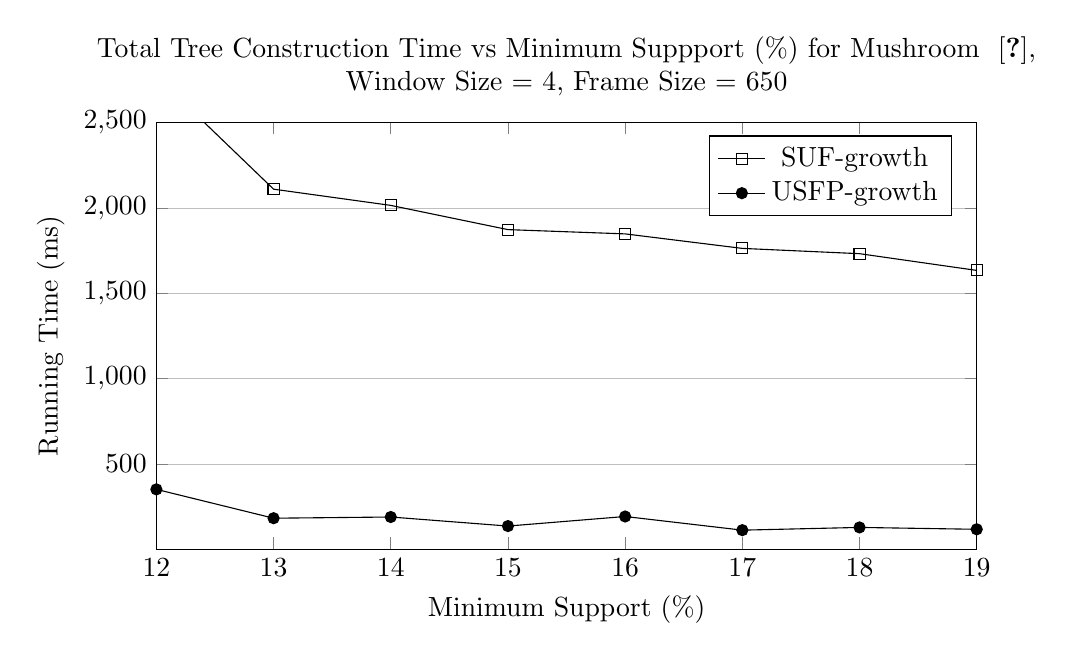
\begin{tikzpicture}
\begin{axis}[
	title={\parbox{\linewidth}{\centering Total Tree Construction Time vs Minimum Suppport (\%) for Mushroom ~\cite{dataset}, Window Size = 4, Frame Size = 650}},
	width=12cm,
	height=7cm,
    xlabel={Minimum Support (\%) },
    ylabel={Running Time (ms)},
    xmin=12, xmax=19,
    ymin=0, ymax=2500,
    xtick={12,13,14,15,16,17,18,19},
    ytick={500,1000,1500,2000,2500},
    legend pos=north east,
    ymajorgrids=true,
    grid style={line width=.2pt,draw=gray!50},
]
 
\addplot[
    solid, every mark/.append style={solid, fill=gray}, mark=square
    ]
    coordinates {
	(12,2771)
	(13,2110)
	(14,2015)
	(15,1873)
	(16,1848)
	(17,1763)
	(18,1732)
	(19,1634)
	};
    \addlegendentry{SUF-growth}
\addplot[
    solid, every mark/.append style={solid, fill=black}, mark=*
    ]
    coordinates {
	(12,351)
	(13,182)
	(14,189)
	(15,136)
	(16,192)
	(17,112)
	(18,128)
	(19,117)
};
    \addlegendentry{USFP-growth}
 
\end{axis}
\end{tikzpicture}
%\end{document}
			\caption{Total Tree Construction Time vs Minimum Suppport (\%) for Mushroom Dataset ~\cite{dataset}}
			\label{result:g_m_tree_construction_total}
			\end{figure}
			
			\begin{figure}
			\centering
				%%mark = star, diamond, square, otimes
%\documentclass{article}
%\usepackage{pgfplots}
%\usepackage[justification=centering]{caption}
%\pgfplotsset{compat=newest}
%\begin{document}
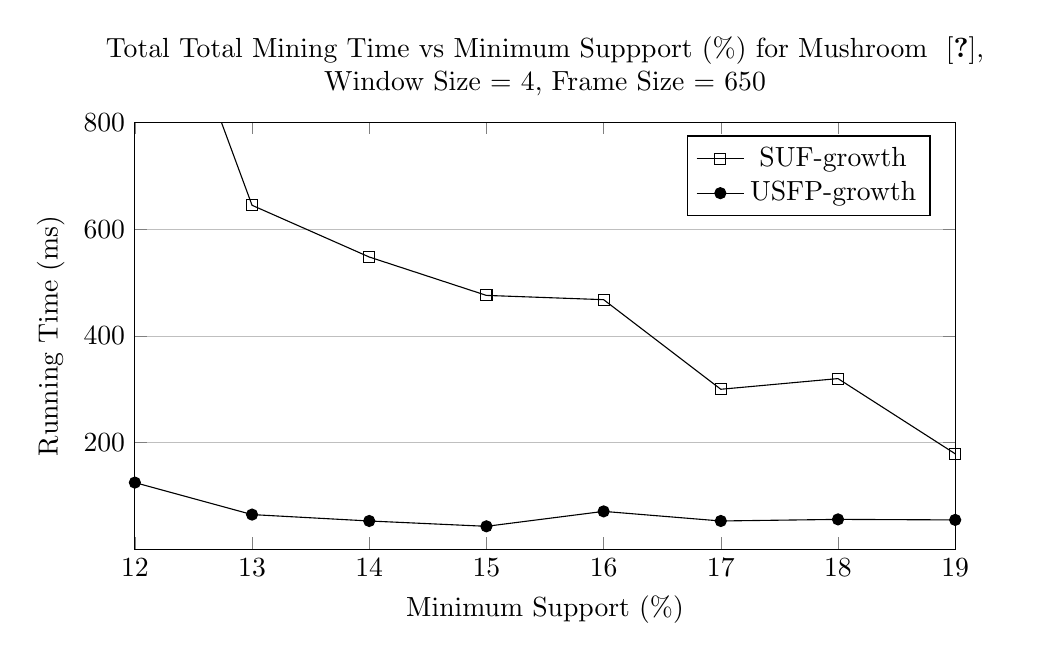
\begin{tikzpicture}
\begin{axis}[
	title={\parbox{\linewidth}{\centering Total Total Mining Time vs Minimum Suppport (\%) for Mushroom ~\cite{dataset}, Window Size = 4, Frame Size = 650}},
	width=12cm,
	height=7cm,
    xlabel={Minimum Support (\%) },
    ylabel={Running Time (ms)},
    xmin=12, xmax=19,
    ymin=0, ymax=800,
    xtick={12,13,14,15,16,17,18,19},
    ytick={200,400,600,800},
    legend pos=north east,
    ymajorgrids=true,
    grid style={line width=.2pt,draw=gray!50},
]
 
\addplot[
    solid, every mark/.append style={solid, fill=gray}, mark=square
    ]
    coordinates {
	(12,1240)
	(13,645)
	(14,548)
	(15,476)
	(16,468)
	(17,300)
	(18,320)
	(19,179)
};
    \addlegendentry{SUF-growth}
\addplot[
    solid, every mark/.append style={solid, fill=black}, mark=*
    ]
    coordinates {
	(12,125)
	(13,65 )
	(14,53 )
	(15,43 )
	(16,71 )
	(17,53 )
	(18,56 )
	(19,55 )
};
    \addlegendentry{USFP-growth}
 
\end{axis}
\end{tikzpicture}
%\end{document}
			\caption{Total Tree Mining Time vs Minimum Suppport (\%) for Mushroom Dataset ~\cite{dataset}}
			\label{result:g_m_mining_total}
			\end{figure}
			
			\begin{figure}
			\centering
				%%mark = star, diamond, square, otimes
%\documentclass{article}
%\usepackage{pgfplots}
%\usepackage[justification=centering]{caption}
%\pgfplotsset{compat=newest}
%\begin{document}
\begin{figure}[!h]
\centering

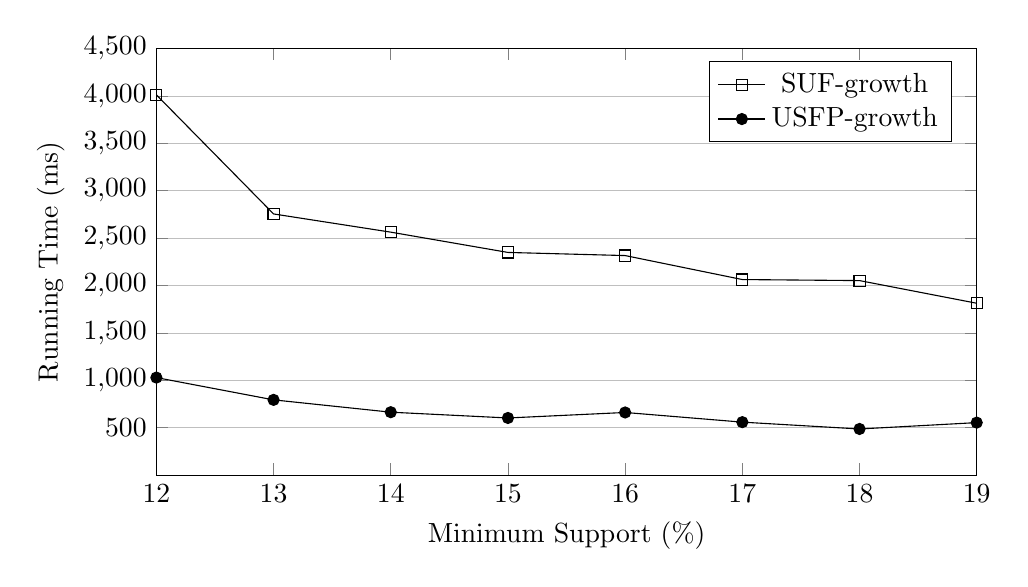
\begin{tikzpicture}
\begin{axis}[
 width=12cm,
   height=7cm,
    xlabel={Minimum Support (\%) },
    ylabel={Running Time (ms)},
    xmin=12, xmax=19,
    ymin=0, ymax=4500,
    xtick={12,13,14,15,16,17,18,19},
    ytick={500,1000,1500,2000,2500,3000,3500,4000,4500},
    legend pos=north east,
    ymajorgrids=true,
    grid style={line width=.2pt,draw=gray!50},
]
 
\addplot[
    solid, every mark/.append style={solid, fill=gray}, mark=square
    ]
    coordinates {
	(12,4011)
	(13,2755)
	(14,2563)
	(15,2349)
	(16,2316)
	(17,2063)
	(18,2052)
	(19,1813)
};
    \addlegendentry{SUF-growth}
\addplot[
    solid, every mark/.append style={solid, fill=black}, mark=*
    ]
    coordinates {
	(12,1029)
	(13,794)
	(14,664)
	(15,603)
	(16,661)
	(17,559)
	(18,487)
	(19,554)
};
    \addlegendentry{USFP-growth}
 
\end{axis}
\end{tikzpicture}
\caption{Total Time (Tree Construction + Mining + False Positive Reduction) vs Minimum Suppport (\%) \\(Window Size = 4, Frame Size = 650) for mushroom database}
\label{result:mushroom_total}
\end{figure}
%\end{document}
			\caption{Running Time vs Minimum Suppport (\%) for Mushroom Dataset ~\cite{dataset}}
			\label{result:g_m_total}
			\end{figure}
					
		\paragraph{T40I10D100K}
		This is Paragraph for T40I10D100K
			\begin{figure}[h]
			\centering
				%%mark = star, diamond, square, otimes
%\documentclass{article}
%\usepackage{pgfplots}
%\usepackage[justification=centering]{caption}
%\pgfplotsset{compat=newest}
%\begin{document}
\begin{figure}
\centering

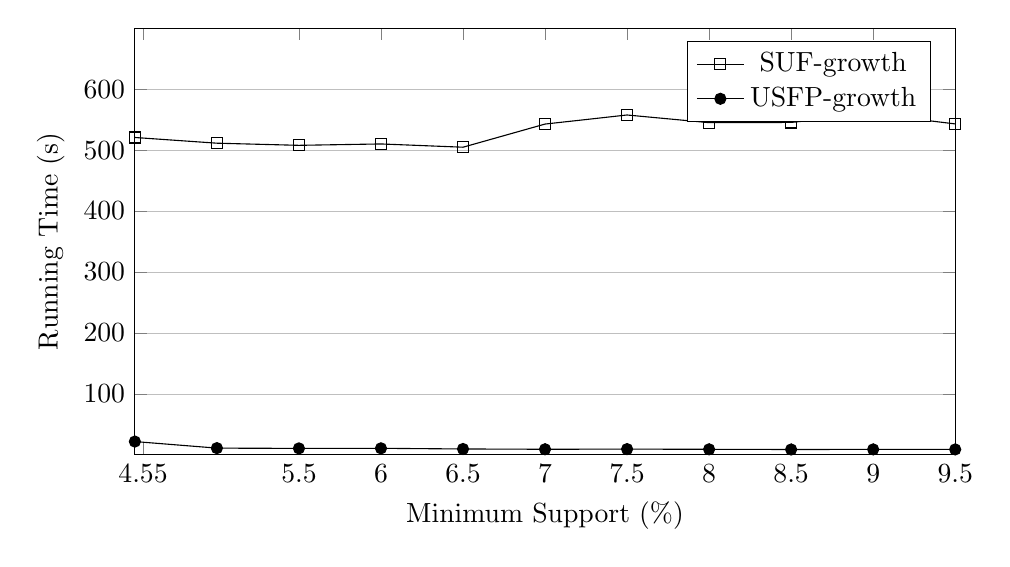
\begin{tikzpicture}
\begin{axis}[
 width=12cm,
   height=7cm,
    xlabel={Minimum Support (\%) },
    ylabel={Running Time (s)},
    xmin=4.5, xmax=9.5,
    ymin=0, ymax=700,
    xtick={4.55,5.5,6,6.5,7,7.5,8,8.5,9,9.5},
    ytick={100,200,300,400,500,600},
    legend pos=north east,
    ymajorgrids=true,
    grid style={line width=.2pt,draw=gray!50},
]
 
\addplot[
    solid, every mark/.append style={solid, fill=gray}, mark=square
    ]
    coordinates {
			(4.5,520.723)
			(5  ,511.365)
			(5.5,507.854)
			(6  ,510.12 )
			(6.5,504.767)
			(7  ,542.742)
			(7.5,557.633)
			(8  ,545.039)
			(8.5,545.444)
			(9  ,559.335)
			(9.5,542.996)

	};
    \addlegendentry{SUF-growth}
\addplot[
    solid, every mark/.append style={solid, fill=black}, mark=*
    ]
    coordinates {
		(4.5,21.814)
		(5  ,11.035)
		(5.5,10.601)
		(6  ,10.723)
		(6.5,9.646 )
		(7  ,9.177 )
		(7.5,9.427 )
		(8  ,9.092 )
		(8.5,8.8   )
		(9  ,8.95  )
		(9.5,8.883 )

};
    \addlegendentry{USFP-growth}
 
\end{axis}
\end{tikzpicture}
\caption{Total Tree Construction Time vs Minimum Suppport (\%) (Window Size = 5, Frame Size = 7000) for T40I10D100K database}
\label{result:t10_tree_total}
\end{figure}
%\end{document}
			\caption{Total Tree Construction Time vs Minimum Suppport (\%) for T40I10D100K Dataset ~\cite{dataset}}
			\label{result:g_t10_tree_construction_total}
			\end{figure}
			
			\begin{figure}
			\centering
				%%%mark = star, diamond, square, otimes
%\documentclass{article}
%\usepackage{pgfplots}
%\usepackage[justification=centering]{caption}
%\pgfplotsset{compat=newest}
%\begin{document}
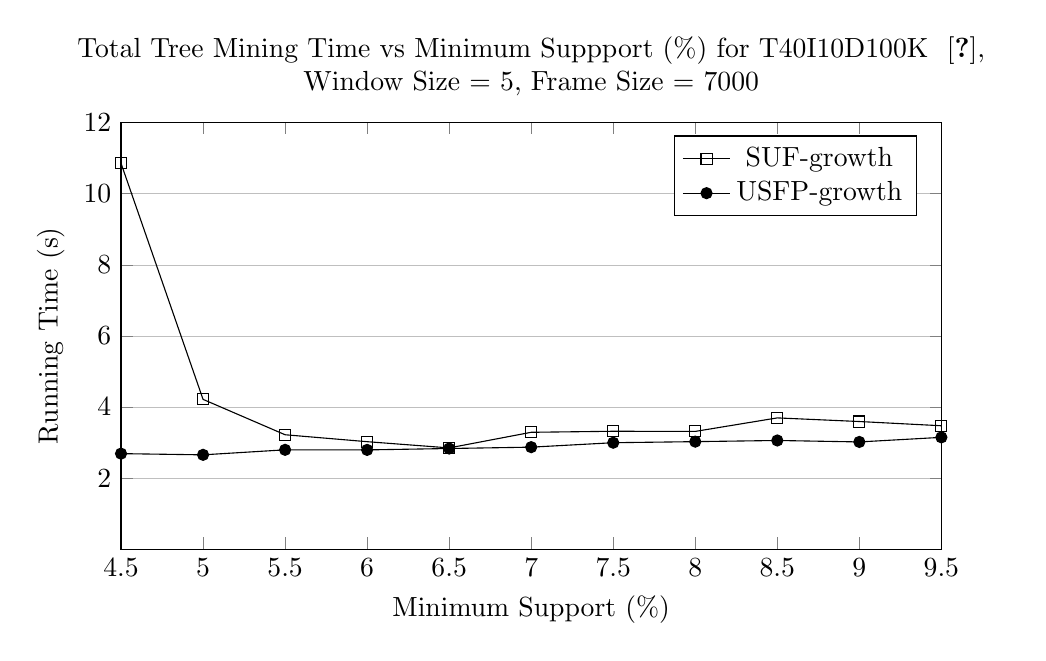
\begin{tikzpicture}
\begin{axis}[
	title={\parbox{\linewidth}{\centering Total Tree Mining Time vs Minimum Suppport (\%) for T40I10D100K ~\cite{dataset}, Window Size = 5, Frame Size = 7000}},
	width=12cm,
	height=7cm,
    xlabel={Minimum Support (\%) },
    ylabel={Running Time (s)},
    xmin=4.5, xmax=9.5,
    ymin=0, ymax=12,
    xtick={4.5,5,5.5,6,6.5,7,7.5,8,8.5,9,9.5},
    ytick={2,4,6,8,10,12},
    legend pos=north east,
    ymajorgrids=true,
    grid style={line width=.2pt,draw=gray!50},
]
 
\addplot[
    solid, every mark/.append style={solid, fill=gray}, mark=square
    ]
    coordinates {
			(4.5,10.856)
			(5  ,4.216 )
			(5.5,3.221 )
			(6  ,3.026 )
			(6.5,2.851 )
			(7  ,3.29  )
			(7.5,3.319 )
			(8  ,3.315 )
			(8.5,3.695 )
			(9  ,3.593 )
			(9.5,3.474 )

};
    \addlegendentry{SUF-growth}
\addplot[
    solid, every mark/.append style={solid, fill=black}, mark=*
    ]
    coordinates {
			(4.5,2.69  )
			(5  ,2.656 )
			(5.5,2.797 )
			(6  ,2.795 )
			(6.5,2.834 )
			(7  ,2.872 )
			(7.5,2.997 )
			(8  ,3.027 )
			(8.5,3.06  )
			(9  ,3.019 )
			(9.5,3.148 )

};
    \addlegendentry{USFP-growth}
 
\end{axis}
\end{tikzpicture}
%\end{document}
			\caption{Total Tree Mining Time vs Minimum Suppport (\%) for T40I10D100K Dataset ~\cite{dataset}}
			\label{result:g_t10_mining_total}
			\end{figure}
			
			\begin{figure}
			\centering
				%%%mark = star, diamond, square, otimes
%\documentclass{article}
%\usepackage{pgfplots}
%\usepackage[justification=centering]{caption}
%\pgfplotsset{compat=newest}
%\begin{document}
\begin{figure}
\centering

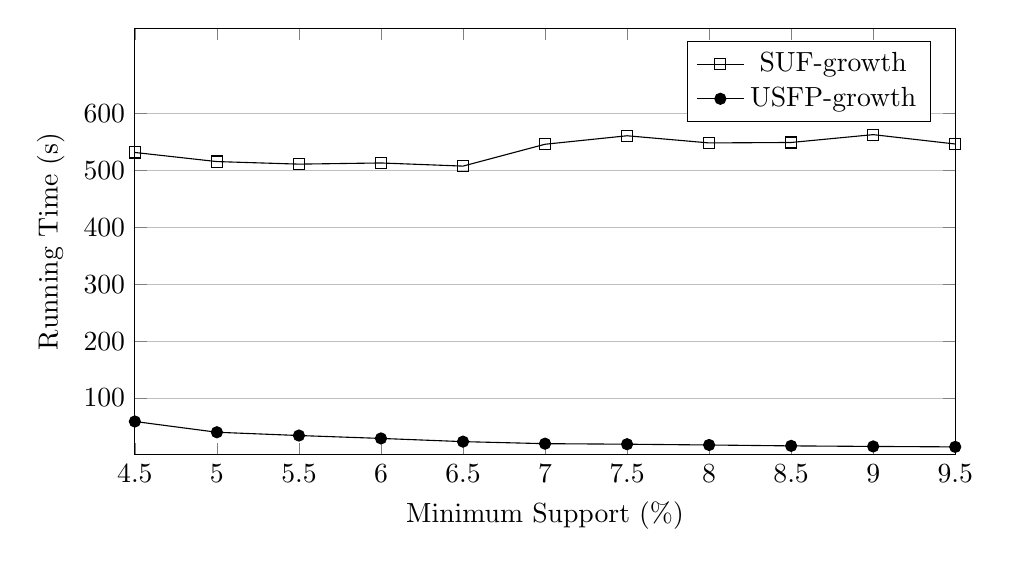
\begin{tikzpicture}
\begin{axis}[
 width=12cm,
   height=7cm,
    xlabel={Minimum Support (\%) },
    ylabel={Running Time (s)},
    xmin=4.5, xmax=9.5,
    ymin=0, ymax=750,
    xtick={4.5,5,5.5,6,6.5,7,7.5,8,8.5,9,9.5},
    ytick={100,200,300,400,500,600},
    legend pos=north east,
    ymajorgrids=true,
    grid style={line width=.2pt,draw=gray!50},
]
 
\addplot[
    solid, every mark/.append style={solid, fill=gray}, mark=square
    ]
    coordinates {
			(4.5,531.579)
			(5  ,515.581)
			(5.5,511.075)
			(6  ,513.146)
			(6.5,507.618)
			(7  ,546.032)
			(7.5,560.952)
			(8  ,548.354)
			(8.5,549.139)
			(9  ,562.928)
			(9.5,546.47 )

};
    \addlegendentry{SUF-growth}
\addplot[
    solid, every mark/.append style={solid, fill=black}, mark=*
    ]
    coordinates {
			(4.5,58.652)
			(5  ,39.735)
			(5.5,33.993)
			(6  ,28.892)
			(6.5,23.262)
			(7  ,19.669)
			(7.5,18.735)
			(8  ,17.355)
			(8.5,15.785)
			(9  ,14.803)
			(9.5,14.013)

};
    \addlegendentry{USFP-growth}
 
\end{axis}
\end{tikzpicture}
\caption{Total Time (Tree Construction + Mining + False Positive Reduction) vs Minimum Suppport (\%) (Window Size = 5, Frame Size = 7000) for T40I10D100K database}
\label{result:t10_total}
\end{figure}
%\end{document}
			\caption{Running Time vs Minimum Suppport (\%) for T40I10D100K Dataset ~\cite{dataset}}
			\label{result:g_t10_total}
			\end{figure}
		
		\paragraph{Chess}
		
			\begin{figure}[h]
			\centering
				\input{result/chess/g_chess_tree_construction_total}
			\caption{Total Tree Construction Time vs Minimum Suppport (\%) for Chess Dataset ~\cite{dataset}}
			\label{result:g_chess_tree_construction_total}
			\end{figure}
			
			\begin{figure}
			\centering
				\input{result/chess/g_chess_mining_total}
			\caption{Total Tree Mining Time vs Minimum Suppport (\%) for Chess Dataset ~\cite{dataset}}
			\label{result:g_chess_mining_total}
			\end{figure}
			
			\begin{figure}
			\centering
				\input{result/chess/g_chess_total}
			\caption{Running Time vs Minimum Suppport (\%) for Chess Dataset ~\cite{dataset}}
			\label{result:g_chess_total}
			\end{figure}

\clearpage		
	\subsubsection{Memory Comparison}
		As our proposed \emph{US-tree} have capability to share nodes more than \emph{SUF-grouwth} ~\cite{dataset}, we get much more gain in memory. The experimental result also indicates that very clearly. Figure \ref{result:g_m_memory_node} shows the memory comparison on mushroom dataset. Mushroom is dense database so we get  much more gain in memory. The graph clearly shows that with the increase of total transaction in the tree gives the much more gain. For chess dataset the the compactness of tree is also very impressive as this dataset is also compact (figure \ref{result:g_chess_memory_node}) the Dense dataset have more scope to share nodes more. Figure \ref{result:g_t10_memory_node} also shows that in T40I10D100K database we also gain the memory optimization. As the database is sparse, we get the memory gain less then dense one.
			\begin{figure}[h]
			\centering
				%%mark = star, diamond, square, otimes
%\documentclass{article}
%\usepackage{pgfplots}
%\usepackage[justification=centering]{caption}
%\pgfplotsset{compat=newest}
%\begin{document}
\begin{figure}[!h]
\centering

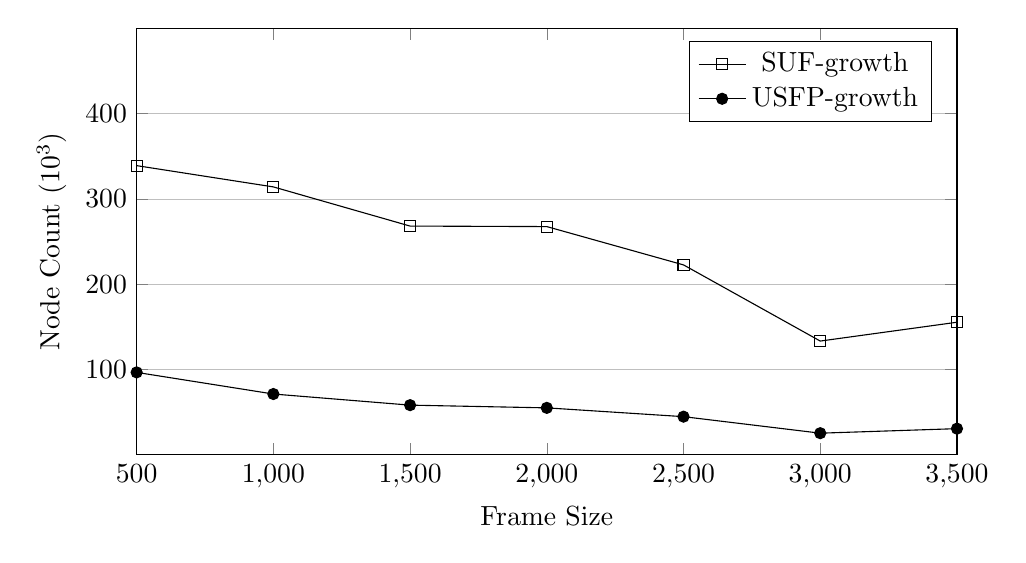
\begin{tikzpicture}
\begin{axis}[
 width=12cm,
   height=7cm,
    xlabel={Frame Size },
    ylabel={Node Count ($10^3$)},
    xmin=500, xmax=3500,
    ymin=0, ymax=500,
    xtick={500,1000,1500,2000,2500,3000,3500},
    ytick={100,200,300,400},
    legend pos=north east,
    ymajorgrids=true,
    grid style={line width=.2pt,draw=gray!50},
]
 
\addplot[
    solid, every mark/.append style={solid, fill=gray}, mark=square
    ]
    coordinates {
			(500,338.966)
			(1000,314.038)
			(1500,268.135)
			(2000,267.525)
			(2500,222.626)
			(3000,133.377)
			(3500,155.435)



	};
    \addlegendentry{SUF-growth}
\addplot[
    solid, every mark/.append style={solid, fill=black}, mark=*
    ]
    coordinates {
			(500,96.670 )
			(1000,71.314)
			(1500,58.275)
			(2000,55.086)
			(2500,44.781)
			(3000,25.416)
			(3500,30.727)


};
    \addlegendentry{USFP-growth}
 
\end{axis}
\end{tikzpicture}
\caption{Total Tree Node vs Frame Size \\(Window Size = 2) for T40I10D100K database}
\label{result:mushroom_total_mem_node}
\end{figure}
%\end{document}
			\caption{Avg Tree Node per window vs Frame Size for Mushroom Dataset ~\cite{dataset}}
			\label{result:g_m_memory_node}
			\end{figure}
			
			\begin{figure}[h]
			\centering
				%mark = star, diamond, square, otimes
%\documentclass{article}
%\usepackage{pgfplots}
%\usepackage[justification=centering]{caption}
%\pgfplotsset{compat=newest}
%\begin{document}
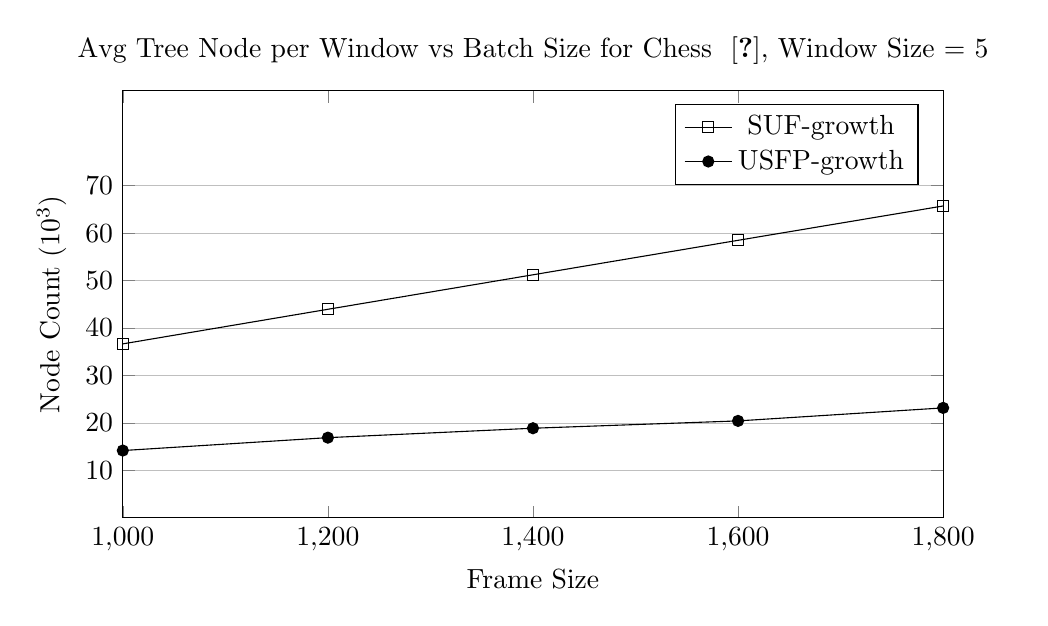
\begin{tikzpicture}
\begin{axis}[
	title={\parbox{\linewidth}{\centering Avg Tree Node per Window vs Batch Size for Chess ~\cite{dataset}, Window Size = 5}},
	width=12cm,
	height=7cm,
    xlabel={Frame Size },
    ylabel={Node Count ($10^3$)},
    xmin=1000, xmax=1800,
    ymin=0, ymax=90,
    xtick={600,800,1000,1200,1400,1600,1800},
    ytick={10,20,30,40,50,60,70},
    legend pos=north east,
    ymajorgrids=true,
    grid style={line width=.2pt,draw=gray!50},
]
 
\addplot[
    solid, every mark/.append style={solid, fill=gray}, mark=square
    ]
    coordinates {
			(600,	22.017)
			(800,	29.326)
			(1000,	36.642)
			(1200,	43.941)
			(1400,	51.218)
			(1600,	58.491)
            (1800,	65.733)



	};
    \addlegendentry{SUF-growth}
\addplot[
    solid, every mark/.append style={solid, fill=black}, mark=*
    ]
    coordinates {
			(600,	8.729)
			(800,	11.074)
			(1000,	14.142)
			(1200,	16.863)
			(1400,	18.849)
			(1600,	20.396)
            (1800,	23.139)


};
    \addlegendentry{USFP-growth}
 
\end{axis}
\end{tikzpicture}
%\end{document}
			\caption{Avg Tree Node per window vs Frame Size for Chess Dataset ~\cite{dataset}}
			\label{result:g_chess_memory_node}
			\end{figure}
			
			\begin{figure}[h]
				%%mark = star, diamond, square, otimes
%\documentclass{article}
%\usepackage{pgfplots}
%\usepackage[justification=centering]{caption}
%\pgfplotsset{compat=newest}
%\begin{document}
\begin{figure}[!h]
\centering

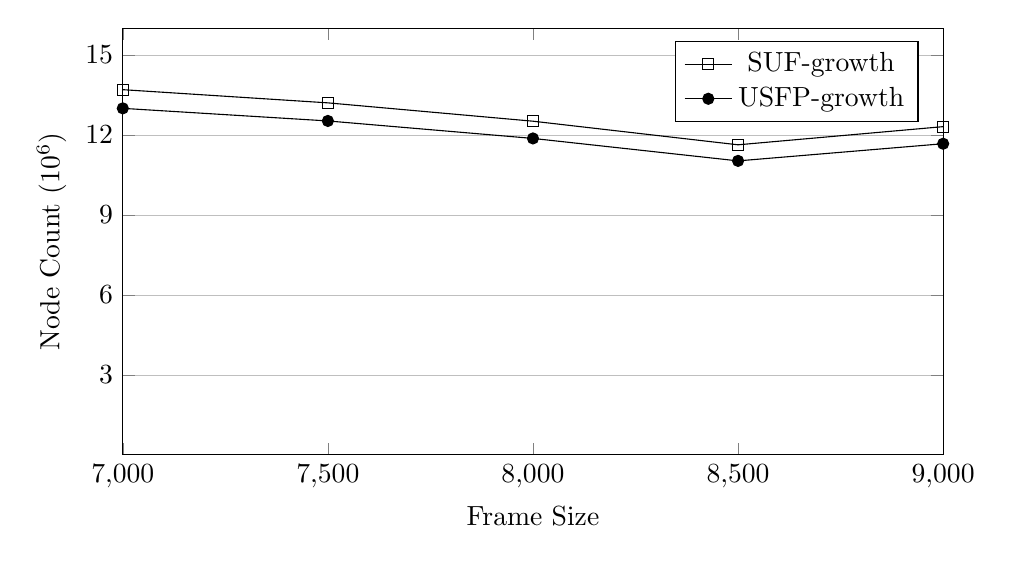
\begin{tikzpicture}
\begin{axis}[
 width=12cm,
   height=7cm,
    xlabel={Frame Size },
    ylabel={Node Count ($10^6$)},
    xmin=7000, xmax=9000,
    ymin=0, ymax=16,
    xtick={7000,7500,8000,8500,9000},
    ytick={3,6,9,12,15},
    legend pos=north east,
    ymajorgrids=true,
    grid style={line width=.2pt,draw=gray!50},
]
 
\addplot[
    solid, every mark/.append style={solid, fill=gray}, mark=square
    ]
    coordinates {
		(7000,13.695556)
		(7500,13.200902)
		(8000,12.512976)
		(8500,11.627701)
		(9000,12.308889)
		(9500,11.134408)


	};
    \addlegendentry{SUF-growth}
\addplot[
    solid, every mark/.append style={solid, fill=black}, mark=*
    ]
    coordinates {
			(7000,12.995104)
			(7500,12.522495)
			(8000,11.867025)
			(8500,11.024889)
			(9000,11.668386)
			(9500,10.552641)

};
    \addlegendentry{USFP-growth}
 
\end{axis}
\end{tikzpicture}
\caption{Total Tree Node vs Frame Size\\(Window Size = 5) for T40I10D100K database}
\label{result:t10_total_mem_node}
\end{figure}
%\end{document}
			\caption{Avg Tree Node per window vs Frame Size for T40I10D100K Dataset ~\cite{dataset}}
			\label{result:g_t10_memory_node}
			\end{figure}
		

\clearpage
\section{Summary}
In summary, our proposed \emph{US-tree}, construction \emph{USFP-growth} mining algorithm is very correct, efficient, the scalable algorithm that works fine in any configuration (minimum support, window size, batch size). For dense dataset (both real and synthetic) this is very efficient. For sparse dataset, this also gives us gain both in memory and in running time. The \emph{U\textsuperscript{cap}} value gives much more benefit to share nodes in the \emph{US-tree}. The compactness of \emph{US-tree} is surprisingly noticeable. Mining compact \emph{US-tree} gives the main surprise in the running time. The \emph{USFP-growth} mining algorithm works nicely without generating no false negatives and a little amount of false positives that can efficiently be removed using the false positive reduction technique.
%
%\end{document}